%%%%%%%%%%%%%%%%%%%%%%%%%%%%%%%%%%%%%%%%%%%%%%%%%%%%%%%%%%%%%%%
%
% Welcome to Overleaf --- just edit your LaTeX on the left,
% and we'll compile it for you on the right. If you open th
%%%%%%%%%%%%%%%%%%%%%%%%%%%%%%%%%%%%%%%%%%%%%%%%%%%%%%%%%%%%%%%
% ------------ CẤU HÌNH TÀI LIỆU ------------

\documentclass[a4paper,12pt]{report}

% ---------- Encoding & Ngôn ngữ ----------
\usepackage[utf8]{inputenc}
\usepackage[vietnamese]{babel}

% ---------- Toán học & Hình ảnh ----------
\usepackage{amsmath}
\usepackage{graphicx}
\usepackage{tikz}
\usetikzlibrary{shapes,arrows,positioning}

% ---------- Danh sách & Bố trí ----------
\usepackage{enumitem}
\usepackage{multicol}
\usepackage{wrapfig}
\usepackage{float}

% ---------- Caption & Liên kết ----------
\usepackage[font=small,labelfont=bf]{caption}
\usepackage{hyperref}

% ---------- Bảng biểu ----------
\usepackage{array}
\usepackage{booktabs}
\usepackage{tabularx}

% ---------- Hiển thị đoạn code ----------
\usepackage{verbatim}
\usepackage{fancyvrb}

% ---------- Tùy chỉnh trình bày ----------
\usepackage{geometry}
\geometry{
	top=2.5cm,
	bottom=2.5cm,
	left=2.5cm,
	right=2.5cm
}
\usepackage{setspace}
\onehalfspacing

% ---------- Tùy chỉnh header & footer ----------
\usepackage{titlesec}
\usepackage{fancyhdr}
\pagestyle{fancy}
\fancyhf{}
\fancyhead[L]{\leftmark}      % Hiển thị tiêu đề chương ở đầu trang bên trái
\fancyfoot[C]{\thepage}       % Số trang ở giữa chân trang
\renewcommand{\headrulewidth}{0.4pt}   % Đường kẻ đầu trang
\renewcommand{\footrulewidth}{0pt}     % Không có đường kẻ chân trang

% Hiển thị "Chương X Tên chương" trong header
\renewcommand{\chaptermark}[1]{\markboth{Chương \thechapter\quad #1}{}}

% ---------- Tùy chỉnh đoạn văn ----------
\setlength{\parindent}{0pt}    % Không thụt đầu dòng các đoạn
\setlength{\parskip}{1em}      % Khoảng cách giữa các đoạn
\usepackage{indentfirst}       % Thụt đầu dòng đoạn đầu tiên mỗi chương

% ---------- Ẩn đánh số trang ở trang bìa ----------
\usepackage{etoolbox}
\AtBeginDocument{\thispagestyle{empty}}  % Trang đầu không có số trang



\begin{document}
% Trang bìa
\thispagestyle{empty}
\begin{center}
	% Khung viền màu xanh dương - CHỈ VIỀN CÓ MÀU
	\setlength{\fboxrule}{2pt} % Độ dày viền 2pt
	\setlength{\fboxsep}{20pt} % Khoảng cách từ viền đến nội dung
	
	% Tạo viền màu xanh dương - chỉ viền, nội dung vẫn màu đen
	\fcolorbox{darkblue}{white}{%
		\begin{minipage}{0.9\textwidth}
			\vspace{1cm}
			\begin{center}
				\textbf{ĐẠI HỌC QUỐC GIA TP. HỒ CHÍ MINH} \\[0.2cm]
				\textbf{TRƯỜNG ĐẠI HỌC BÁCH KHOA} \\[0.2cm]
				\textbf{KHOA ĐIỆN - ĐIỆN TỬ} \\[0.2cm]
				-----------------o0o----------------- \\[0.5cm]
				
				% Logo placeholder
				\vspace{0.5cm}
				
\includegraphics[height=5cm]{logo-hcmut.png}
				\vspace{1cm} % Khoảng cách sau logo
				
				\textbf{BÁO CÁO ĐỒ ÁN MÔN HỌC 2} \\[1cm]
				
				\textbf{ĐỀ TÀI: THIẾT BỊ ĐEO PHÁT HIỆN TÉ NGÃ CHO NGƯỜI CAO TUỔI VÀ BỆNH NHÂN} \\[0.3cm]
				\textit{Fall Detection and Alert Wearable Device for The Elderly and Patients} \\[1cm]
				
				\textbf{GVHD:} PGS. TS Hà Hoàng Kha \\[0.2cm]
				\textbf{SVTH:} Trần Đức Hảo \\[0.2cm]
				\textbf{MSSV:} 1734011\\[1cm]
				
				\textbf{TP. HỒ CHÍ MINH, THÁNG 05 NĂM 2025}
			\end{center}
			\vspace{1cm}
		\end{minipage}
	}
\end{center}

\newpage

	% TRANG NHIỆM VỤ-----------------------------------------------------------
	\thispagestyle{empty}
	
	\setstretch{0.8} % Thu nhỏ khoảng cách dòng
	
	% ===== PHẦN TIÊU ĐỀ VÀ NỘI DUNG CHÍNH =====
	% Tiêu đề đầu trang
	\noindent
	\begin{minipage}[t]{0.48\textwidth}
		\centering
		\textbf{ĐẠI HỌC QUỐC GIA TP.HCM} \\
		\textbf{TRƯỜNG ĐẠI HỌC BÁCH KHOA} \\
	\end{minipage}%
	\hfill
	\begin{minipage}[t]{0.48\textwidth}
		\centering
		\textbf{CỘNG HOÀ XÃ HỘI CHỦ NGHĨA VIỆT NAM} \\
		\textbf{Độc lập -- Tự do -- Hạnh phúc} \\
	\end{minipage}
	
	\vspace{0.5em}
	
	% Thông tin đầu trang
	\noindent
	\begin{tabular}{ll}
		Số: & \underline{\hspace{2cm}}/BK-ĐPT \\
		Khoa: & Điện -- Điện tử \\
		Bộ Môn: & Viễn Thông \\
	\end{tabular}
	
	\vspace{0.5em}
	
	% Tiêu đề chính
	\begin{center}
		\textbf{\large NHIỆM VỤ ĐỒ ÁN MÔN HỌC 2}
	\end{center}
	
	\vspace{0.5em}
	
	% Thông tin sinh viên và đề tài
	\noindent
	\begin{tabular}{ll}
		1. Họ và tên: & Trần Đức Hảo \hspace{2cm} MSSV: 1734011 \\
		2. Ngành: & Điện tử - Viễn Thông \\
		3. Đề tài: & Thiết Bị Đeo Phát Hiện Té Ngã Cho Người Cao Tuổi Và Bệnh Nhân \\
		4. Nhiệm vụ: \\
		
		
	\end{tabular}
	
	\vspace{0.5em}
	
	% Ngày tháng và hướng dẫn
	\noindent
	5. Ngày giao nhiệm vụ đồ án môn học 2: \dotfill
	
	\noindent
	6. Ngày hoàn thành nhiệm vụ: \dotfill
	
	\noindent
	7. Họ và tên người hướng dẫn: PGS. TS Hà Hoàng Kha
	
	\vspace{0.5em}
	
	\noindent
	Nội dung và yêu cầu đồ án môn học 2 đã được thông qua Bộ Môn.
	
	\vspace{0.5em}
	
	\noindent
	TP. HCM, ngày \dotfill tháng \dotfill năm 2025
	
	\vspace{1em}
	
	% Phần chữ ký
	\noindent
	\begin{tabular}{
			@{}
			>{\centering\arraybackslash}p{0.45\textwidth}
			@{\hspace{0.1\textwidth}}
			>{\centering\arraybackslash}p{0.45\textwidth}
			@{}
		}
		\textbf{CHỦ NHIỆM BỘ MÔN} & \textbf{NGƯỜI HƯỚNG DẪN CHÍNH} \\
		& \\[1.5cm]
		\textbf{(Ký và ghi rõ họ tên)} & \textbf{(Ký và ghi rõ họ tên)}
	\end{tabular}
	
	\vspace{2em}
	
	% ===== PHẦN DÀNH CHO KHOA/BỘ MÔN (Đặt ở cuối) =====
	
	% Phần dành cho khoa bộ môn (nửa trái văn bản)
	\noindent
	\begin{minipage}[t]{0.5\textwidth}
		\textbf{\makebox[\linewidth][l]{PHẦN DÀNH CHO KHOA, BỘ MÔN:}} % Đảm bảo nằm trên 1 dòng
		\vspace{0.5em}
		
		\begin{tabular}{@{} p{\linewidth} @{}}
			Người duyệt (chấm sơ bộ): \dotfill \\[0.3cm]
			Ngày ký: \dotfill \\[0.3cm]
			Điểm đánh giá: \dotfill \\[0.3cm]
			Nhận xét: \dotfill \\[0.3cm]
			\dotfill \\[0.3cm]
			Lưu tại bộ môn: \dotfill \\
		\end{tabular}
	\end{minipage}%
	\newpage
	% trang lời cảm ơn
	\cleardoublepage  % Bắt đầu trang mới bên phải (nếu dùng twoside)
	\thispagestyle{empty}  % Tắt header/footer
	
	\begin{center}
		\vspace*{3cm}  % Cách mép trên 3cm
		
		\textbf{\fontsize{16}{19}\selectfont LỜI CẢM ƠN}
		
		\vspace{2cm}  % Khoảng cách sau tiêu đề
	\end{center}
	
	\noindent
	\begin{minipage}{\linewidth}
		\setlength{\parindent}{1.5cm}  % Thụt đầu dòng 1.5cm
		\setlength{\parskip}{6pt}      % Dãn dòng 6pt
		\fontsize{13}{15}\selectfont   % Cỡ chữ 13pt, dãn dòng 15pt
		
		Trước hết, tôi xin bày tỏ lòng biết ơn sâu sắc đến \textbf{PGS.TS. Hà Hoàng Kha}, người đã tận tình hướng dẫn, chỉ bảo tôi trong suốt quá trình nghiên cứu và hoàn thành luận văn này.
		
		Tôi trân trọng cảm ơn các thầy cô trong \textbf{Bộ môn Viễn Thông}, \textbf{Khoa Điện - Điện tử}, \textbf{Trường Đại học Bách Khoa TP.HCM} đã trang bị cho tôi kiến thức nền tảng và tạo điều kiện thuận lợi cho quá trình học tập.
		
		
		\vspace{1.5cm}
		\begin{flushright}
			\begin{minipage}{0.5\textwidth}
				\centering
				\textit{Tp. Hồ Chí Minh, ngày ...... tháng ...... năm 2025} \\
				\vspace{1cm}
				\textbf{Sinh Viên} \\
				\vspace{0.5cm}
				\textbf{Trần Đức Hảo}
			\end{minipage}
		\end{flushright}
	\end{minipage}
	
	\vfill
	\newpage
	
	% muc luc-------------
	\begingroup
	\let\clearpage\relax
	\setcounter{tocdepth}{1}
	\tableofcontents
	\endgroup
	
	\clearpage
	\pagenumbering{arabic}
	\clearpage
	
	% trang tóm tắt ----------------------------
	
	
	\begin{center}
		\textbf{TÓM TẮT ĐỀ TÀI: THIẾT BỊ ĐEO PHÁT HIỆN TÉ NGÃ CHO NGƯỜI CAO TUỔI VÀ BỆNH NHÂN}
	\end{center}
	\setlength{\parindent}{1cm}
	
	Báo cáo này trình bày quá trình thiết kế và triển khai một hệ thống cảnh báo té ngã dành cho người cao tuổi và bệnh nhân, sử dụng vi điều khiển ESP32, cảm biến gia tốc MPU6050 và module 4G-GPS Quectel EC800K. Hệ thống có khả năng phát hiện té ngã và gửi tin nhắn SMS chứa tọa độ GPS đến số điện thoại đã được thiết lập sẵn. Toàn bộ hệ thống được xây dựng trên nền tảng ESP-IDF, chia thành nhiều tác vụ (task) hoạt động song song dựa trên FreeRTOS.
	
	Lý do chọn đề tài xuất phát từ đề xuất của giảng viên hướng dẫn, đồng thời nhận thấy tính ứng dụng cao của hệ thống trong đời sống thực tế. Thiết bị hỗ trợ người dùng gặp khó khăn trong vận động có thể sinh hoạt độc lập, đồng thời giúp người thân và người chăm sóc theo dõi kịp thời khi xảy ra sự cố. Trong quá trình thực hiện, đề tài kết hợp nhiều thiết bị ngoại vi như cảm biến và module truyền thông, giúp sinh viên rèn luyện kỹ năng tích hợp phần cứng và phần mềm, đồng thời củng cố kiến thức lý thuyết đã học. Ngoài ra, hệ thống còn có tiềm năng mở rộng, như tích hợp vào hệ sinh thái chăm sóc sức khỏe thông minh hoặc nền tảng IoT.
	
	Mục tiêu của đồ án gồm:
	\begin{itemize}
		\item Thiết kế thiết bị đeo có khả năng phát hiện té ngã thông qua cảm biến gia tốc
		\item Gửi cảnh báo khẩn cấp qua SMS hoặc Internet sử dụng module SIM 4G
		\item Định vị vị trí người dùng dựa trên dữ liệu GPS tại thời điểm phát hiện sự cố
		\item Có thể tích hợp thêm chức năng cảnh báo âm thanh tại chỗ để người xung quanh dễ dàng nhận biết và hỗ trợ
	\end{itemize}
	\newpage
	
	% CHƯƠNG 1 GIOI THIEU---------------------------------------------------
	\chapter{GIỚI THIỆU}
	
	
	\section{Tổng quan về vấn đề té ngã}
	
	Té ngã là một trong những nguyên nhân hàng đầu gây chấn thương nghiêm trọng trên toàn cầu, đặc biệt đối với người cao tuổi. Theo Tổ chức Y tế Thế giới (WHO), mỗi năm có khoảng 646.000 ca tử vong do té ngã, khiến nó trở thành nguyên nhân gây tử vong hàng đầu do tai nạn ngoài ý muốn. Thống kê cho thấy nhóm đối tượng có nguy cơ cao nhất là người trên 65 tuổi, với tỷ lệ té ngã hơn 30\% mỗi năm, và tỷ lệ này tăng lên đến 50\% đối với người trên 80 tuổi. Tại Việt Nam, vấn đề này ngày càng trở nên cấp bách do tốc độ già hóa dân số diễn ra nhanh chóng. Theo số liệu từ Tổng cục Thống kê, tỷ lệ người cao tuổi (trên 60 tuổi) hiện chiếm khoảng 12\% tổng dân số và dự kiến sẽ tăng lên 25\% vào năm 2049. Điều này đặt ra những thách thức lớn cho hệ thống y tế trong việc giải quyết các vấn đề liên quan đến té ngã ở người cao tuổi.
	
	Hậu quả của té ngã không chỉ bao gồm các tổn thương thể chất như gãy xương hay chấn thương đầu, mà còn gây ra những ảnh hưởng tâm lý nghiêm trọng, chẳng hạn như hội chứng sợ té ngã, dẫn đến hạn chế vận động và suy giảm chất lượng cuộc sống. Đáng lo ngại hơn là những trường hợp té ngã xảy ra khi nạn nhân ở một mình và không thể tự gọi cứu trợ. Trong những tình huống này, việc nằm lâu trên sàn mà không được hỗ trợ kịp thời có thể dẫn đến các biến chứng nguy hiểm như hạ thân nhiệt, mất nước, nhiễm trùng, thậm chí tử vong. Công nghệ phát hiện té ngã tự động đóng vai trò quan trọng trong việc giảm thiểu hậu quả nghiêm trọng này. Các hệ thống này hoạt động dựa trên nguyên lý phát hiện chuyển động bất thường của cơ thể thông qua các cảm biến tiên tiến như gia tốc kế, con quay hồi chuyển và cảm biến áp suất. Khi phát hiện dấu hiệu té ngã, hệ thống có thể tự động gửi cảnh báo đến người thân hoặc dịch vụ cấp cứu, đồng thời cung cấp thông tin chính xác về vị trí của nạn nhân, giúp rút ngắn thời gian cứu hộ và giảm thiểu biến chứng.
	
	\newpage
	
	\textit{Các ứng dụng thực tế của công nghệ cảnh báo té ngã có thể được triển khai trong nhiều lĩnh vực vd như sau:}
	
	\begin{itemize}
		\item \textbf{Chăm sóc người cao tuổi và y tế}: Hỗ trợ người cao tuổi sống độc lập an toàn tại nhà, giảm áp lực cho người chăm sóc và gia đình. Đồng thời, hệ thống giúp nhân viên y tế theo dõi tình trạng bệnh nhân tại các cơ sở y tế, viện dưỡng lão, đặc biệt là những bệnh nhân mắc các bệnh lý ảnh hưởng đến khả năng vận động như Parkinson, di chứng đột quỵ, hoặc rối loạn thăng bằng.
		
		\item \textbf{An toàn lao động công nghiệp}: Bảo vệ công nhân làm việc một mình trong môi trường nguy hiểm như công trường xây dựng, nhà máy sản xuất, hoặc khu vực khai thác mỏ, nơi việc phát hiện và cứu hộ kịp thời có thể cứu sống tính mạng người lao động.
		
		\item \textbf{Thể thao và hoạt động giải trí}: Giám sát và cảnh báo tai nạn trong quá trình luyện tập hoặc thi đấu, đặc biệt hữu ích cho các môn thể thao mạo hiểm như leo núi, lặn biển, trượt tuyết, hoặc đua xe.
		
	\end{itemize}
	
	\textit{Dựa trên nghiên cứu và phân tích các công nghệ hiện có, các giải pháp phát hiện té ngã có thể được phân thành ba nhóm chính:}
	
	\begin{itemize}
		\item \textbf{Hệ thống dựa trên cảm biến đeo trên người}: Sử dụng các thiết bị nhỏ gọn tích hợp cảm biến gia tốc kế và con quay hồi chuyển. Ưu điểm bao gồm tính di động cao, khả năng hoạt động độc lập, chi phí thấp và phù hợp cho người cao tuổi sống một mình.
		
		\item \textbf{Hệ thống dựa trên camera và thị giác máy tính}: Sử dụng công nghệ xử lý hình ảnh và trí tuệ nhân tạo để phân tích video từ camera giám sát. Mặc dù không yêu cầu người dùng đeo thiết bị, hệ thống này có nhược điểm về chi phí cao, vấn đề riêng tư và phụ thuộc vào góc quay cũng như điều kiện ánh sáng.
		
		\item \textbf{Hệ thống dựa trên cảm biến môi trường}: Sử dụng mạng lưới cảm biến cố định như cảm biến áp suất sàn nhà, cảm biến sóng âm hoặc cảm biến độ rung. Tuy nhiên, giải pháp này bị hạn chế về phạm vi hoạt động và chỉ áp dụng trong khu vực được trang bị sẵn hệ thống.
		
	\end{itemize}
	
	\textit{Sau khi đánh giá ưu nhược điểm của từng giải pháp, khả năng hoạt động liên tục và linh hoạt trong sử dụng. Đồ án tập trung phát triển một hệ thống cảnh báo té ngã hoàn chỉnh với các thành phần chính sau:}
	
	\begin{itemize}
		\item \textbf{Vi điều khiển ESP32}: Đóng vai trò trung tâm xử lý dữ liệu và điều khiển hệ thống.
		\item \textbf{Cảm biến MPU6050}: Cung cấp dữ liệu gia tốc và con quay hồi chuyển để phát hiện chuyển động bất thường.
		\item \textbf{Module 4G-GPS Quecktell800K}: Đảm bảo kết nối mạng di động và xác định vị trí chính xác.
	\end{itemize}
	
	Hệ thống được thiết kế dưới dạng thiết bị đeo nhỏ gọn, có khả năng tự động phát hiện té ngã thông qua phân tích dữ liệu từ cảm biến gia tốc. Khi phát hiện sự cố, thiết bị sẽ gửi tin nhắn cảnh báo kèm tọa độ GPS đến số điện thoại đã đăng ký. Giải pháp này không chỉ đảm bảo hỗ trợ kịp thời trong tình huống khẩn cấp mà còn góp phần nâng cao chất lượng cuộc sống và sự an toàn cho người cao tuổi cũng như các đối tượng có nguy cơ té ngã cao.
	
	
	
	% Tinh hinh nghien cuu trong va ngoai nuoc------------------
	\setlength{\parindent}{1cm}
	\section{Tình hình nghiên cứu trong và ngoài nước}
	
	Phát hiện té ngã là lĩnh vực nghiên cứu quan trọng trong chăm sóc sức khỏe, đặc biệt với người cao tuổi. Hiện có ba phương pháp chính: (1) dựa trên cảm biến đeo, (2) thị giác máy tính, và (3) cảm biến môi trường.
	
	\subsection{Các phương pháp phát hiện té ngã hiện nay}
	
	\begin{itemize}
		\item \textbf{Phương pháp dựa trên cảm biến đeo}: Sử dụng gia tốc kế và con quay hồi chuyển để phát hiện chuyển động bất thường. Nghiên cứu của Casilari et al. [1] cho thấy phương pháp này có độ chính xác cao và dễ triển khai trên thiết bị di động. Tuy nhiên, việc tích hợp thêm cảm biến sinh lý (nhịp tim, huyết áp) làm tăng chi phí và độ phức tạp. Vị trí gắn cảm biến cũng ảnh hưởng đến hiệu suất, như nghiên cứu tại Tokyo Institute of Technology đã chỉ ra.
		
		\item \textbf{Phương pháp thị giác máy tính}: Sử dụng camera để phân tích chuyển động. Camera RGB thông thường đạt 90\% độ chính xác trong điều kiện ánh sáng tốt [2], trong khi camera độ sâu (Kinect, Intel RealSense) tạo mô hình 3D cho kết quả tốt hơn trong đa điều kiện ánh sáng [2]. Camera nhiệt có ưu điểm hoạt động trong bóng tối và bảo vệ quyền riêng tư. Hạn chế chung là chi phí cao và phụ thuộc vào điều kiện ánh sáng, góc quay.
		
		\item \textbf{Phương pháp cảm biến môi trường}: Sử dụng hệ thống cảm biến lắp đặt cố định. Cảm biến áp lực sàn phát hiện té ngã qua mẫu áp lực bất thường nhưng có chi phí lắp đặt cao. Cảm biến radar (như VS373 của Milesight) sử dụng radar 4D 60-GHz và AI đạt độ chính xác 99\% [6], trong khi công nghệ của Vayyar [7] cho phép phát hiện mà không xâm phạm quyền riêng tư. Nhược điểm là giới hạn phạm vi hoạt động.
	\end{itemize}
	\subsection{Các sản phẩm thương mại}
	
	Thị trường hiện có nhiều sản phẩm ứng dụng các phương pháp trên:
	
	\begin{itemize}
		\item \textbf{Thiết bị đeo}: Apple Watch [3] tích hợp phát hiện té ngã và gọi khẩn cấp; Philips Lifeline GoSafe 2 [4] kết hợp GPS để định vị; MobileHelp Solo [5] là thiết bị dạng mặt dây chuyền có nút báo động.
		\item \textbf{Hệ thống giám sát}: Vayyar Home [7] dùng radar 4D không cần camera; ASUS Zenbo Junior [8] là robot hỗ trợ tích hợp AI; Nobi Smart Lamp [9] là đèn thông minh có khả năng phát hiện té ngã.
		\item \textbf{Giải pháp phần mềm}: FallCall Detect sử dụng học máy trên Apple Watch; Essence SmartCare là nền tảng theo dõi sức khỏe đa cảm biến.
	\end{itemize}
	
	\subsection{Xu hướng phát triển các phương pháp phát hiện té ngã}
	Hiện nay, các xu hướng phát triển chính trong lĩnh vực phát hiện té ngã tập trung vào việc ứng dụng học máy và AI để nâng cao độ chính xác, tối ưu hóa năng lượng nhằm kéo dài thời lượng pin, kết hợp đa cảm biến để giảm thiểu báo động giả, cùng với việc xử lý dữ liệu tại thiết bị (Edge Computing) giúp giảm độ trễ và tăng cường tính bảo mật riêng tư cho người dùng.
	
	% CHƯƠNG 2 PHAN LY THUYẾT----------------------------------------
	\chapter{LÝ THUYẾT VỀ HỆ THỐNG PHÁT HIỆN TÉ NGÃ SỬ DỤNG CẢM BIẾN ĐEO}
	Nội dung ở chương này sẽ trình bày về lý thuyết nguyên lý hoạt động của các thành phần phần cứng cấu thành nên hệ thống và phương pháp sử dụng để triển khai phần mềm cũng như sơ đồ hoạt động của nó
	
	\section{Tổng quan về hệ thống phát hiện té ngã sử dụng cảm biến đeo}
	
	
	
	\subsection{Cấu trúc hệ thống, và quy trình hoạt động}
	Hệ thống cảnh báo té ngã được thiết kế dựa trên ba thành phần chính: vi điều khiển ESP32, cảm biến MPU6050 và module SIM 4G/GPS (EC800K). Hệ thống hoạt động theo quy trình khép kín từ thu thập dữ liệu đến cảnh báo khẩn cấp. ESP32 đóng vai trò trung tâm xử lý, có nhiệm vụ thu thập và phân tích dữ liệu từ cảm biến MPU6050 - một cảm biến 6 trục tích hợp gia tốc kế và con quay hồi chuyển để theo dõi chuyển động. Module SIM 4G/GPS EC800K thực hiện hai chức năng quan trọng: xác định vị trí chính xác thông qua GPS, Gửi tin nhắn SMS cảnh báo khi phát hiện sự cố. Toàn bộ hệ thống được cấp nguồn bằng pin lithium để đảm bảo tính di động, phù hợp với nhu cầu sử dụng liên tục.
	
	
	\textit{Quá trình vận hành của hệ thống được chia thành bốn giai đoạn chính:}
	
	\begin{itemize}
		\item \textbf{Thu thập và tiền xử lý dữ liệu}: MPU6050 liên tục ghi nhận các thông số gia tốc và vận tốc góc trên ba trục XYZ. Dữ liệu này được truyền về ESP32 thông qua giao tiếp I2C với tần số lấy mẫu 100Hz, đủ để phát hiện các chuyển động đột ngột.
		
		\newpage 
		
		\item \textbf{Phát hiện té ngã}: Hệ thống áp dụng thuật toán kết hợp hai bước:  Xác định gia tốc đột ngột vượt ngưỡng (thường > 2.5g) và  Kiểm tra trạng thái bất động sau đó. Ngoài phương pháp ngưỡng cơ bản, hệ thống có thể tích hợp thêm các mô hình học máy như Decision Tree để nâng cao độ chính xác trong các trường hợp phức tạp.
		
		
		
		\item \textbf{Xử lý sự kiện}: Khi phát hiện té ngã, hệ thống kích hoạt chuỗi hành động: Phát tín hiệu âm thanh qua buzzer,  Nhấp nháy đèn LED cảnh báo,  Gửi tin nhắn SMS chứa tọa độ GPS đến số điện thoại đã đăng ký.
		
		\item \textbf{Ghi nhận và theo dõi}: Toàn bộ dữ liệu sự kiện bao gồm gia tốc, vận tốc góc, thời gian và vị trí được lưu trữ trên bộ nhớ flash của ESP32. Đồng thời, hệ thống cung cấp cổng UART để theo dõi real-time và debug trong quá trình phát triển.
	\end{itemize}
	
	%------------------------------------------
	
	\section{Thành phần và các thông số phần cứng}
	Sau đây là phần trình bày lý thuyết về phần cứng cấu thành và thông số kỹ thuật nổi bật cùng chức năng của chúng
	\subsection{Vi điều khiển ESP32}
	
	\begin{figure}[h]
		\centering
		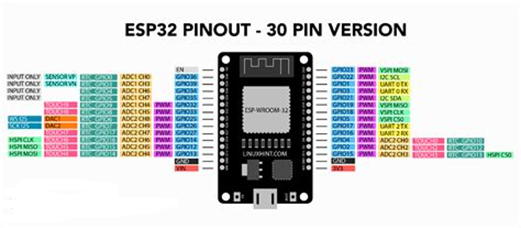
\includegraphics[width=0.5\textwidth]{ESP32_30_PIN.png}
		\caption{Vi điều khiển ESP32}
		\label{fig:esp32}
	\end{figure}
	
	Hình 2.1 trên là hình ảnh mô tả về ESP32 bao gồm chú thích về các chân giao tiếp của chúng là điều khiển mạnh mẽ với các thông số kỹ thuật nổi bật sau:
	
	\begin{itemize}
		\item \textbf{Vi xử lý}:
		\begin{itemize}
			\item CPU: Dual-core hoặc single-core Tensilica LX6, tốc độ 240 MHz
			\item Bộ xử lý tín hiệu: Hỗ trợ DSP cho ứng dụng âm thanh, hình ảnh
		\end{itemize}
		
		\item \textbf{Bộ nhớ}:
		\begin{itemize}
			\item SRAM: 520KB
			\item Flash: 4MB đến 16MB (tùy phiên bản)
		\end{itemize}
		
		\item \textbf{Kết nối không dây}:
		\begin{itemize}
			\item Wi-Fi: 802.11 b/g/n (150Mbps)
			\item Bluetooth: v4.2 BR/EDR và BLE
		\end{itemize}
		
		\item \textbf{Cổng giao tiếp}:
		\begin{itemize}
			\item GPIO: 30+ chân (input/output/PWM/ADC/DAC)
			\item UART: 2 cổng
			\item SPI: 4 cổng
			\item I2C: 2 cổng
		\end{itemize}
		
		\item \textbf{Tính năng đặc biệt}:
		\begin{itemize}
			\item Chế độ "deep sleep" tiết kiệm năng lượng
			\item Tích hợp FreeRTOS cho xử lý đa nhiệm
		\end{itemize}
	\end{itemize}
	
	
	%MPU 6050 ---------------------
	\subsection{Cảm biến MPU6050}
	\begin{figure}[h]
		\centering
		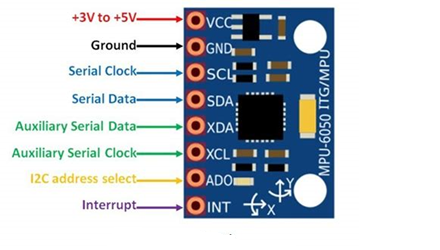
\includegraphics[width=0.5\textwidth]{MPU6050.png}
		\caption{Cảm biến gia tốc và con quay hồi chuyển MPU6050}
		\label{fig:mpu6050}
	\end{figure}
	
	Hình 2.2 trên mô tả MPU6050 và các chân giao tiếp của chúng là cảm biến 6 trục tích hợp gia tốc kế và con quay hồi chuyển với các thông số kỹ thuật sau:
	
	\subsubsection{Thông số kỹ thuật}
	\begin{itemize}
		\item \textbf{Gia tốc kế}:
		\begin{itemize}
			\item Dải đo: ±2g, ±4g, ±8g, ±16g (1g = 9.81 m/s²)
			\item Độ phân giải: 16-bit
			\item Độ nhạy:
			\begin{itemize}
				\item ±2g: 16384 LSB/g
				\item ±4g: 8192 LSB/g
				\item ±8g: 4096 LSB/g
			\end{itemize}
		\end{itemize}
		
		\item \textbf{Con quay hồi chuyển}:
		\begin{itemize}
			\item Dải đo: ±250, ±500, ±1000, ±2000°/s
			\item Độ phân giải: 16-bit
			\item Độ nhạy:
			\begin{itemize}
				\item ±250°/s: 131 LSB/°/s
				\item ±500°/s: 65.5 LSB/°/s
			\end{itemize}
		\end{itemize}
		
		\item \textbf{Điện năng}:
		\begin{itemize}
			\item Điện áp hoạt động: 3.3V
			\item Tiêu thụ năng lượng thấp
		\end{itemize}
		
		\item \textbf{Tính năng đặc biệt}:
		\begin{itemize}
			\item Bộ lọc số low-pass
			\item Chế độ ngủ tiết kiệm năng lượng
		\end{itemize}
	\end{itemize}
	
	\subsubsection{Giao tiếp I2C}
	MPU6050 sử dụng giao thức I2C với cấu trúc:
	\begin{itemize}
		\item SCL (Serial Clock Line): Tín hiệu xung nhịp
		\item SDA (Serial Data Line): Truyền dữ liệu
	\end{itemize}
	
	\begin{table}[h]
		\centering
		\caption{Kết nối MPU6050 với ESP32}
		\label{tab:mpu6050_connection}
		\begin{tabular}{|c|c|c|c|c|}
			\hline
			\textbf{Chân MPU6050} & SDA & SCL & VCC & GND \\ \hline
			\textbf{Chân ESP32} & GPIO21 & GPIO22 & 3.3V & GND \\ \hline
		\end{tabular}
	\end{table}
	
	\subsubsection{Cấu hình phần mềm}
	\begin{itemize}
		\item Sử dụng thư viện \texttt{Wire.h} hoặc \texttt{MPU6050.h}
		\item Quy trình giao tiếp:
		\begin{enumerate}
			\item ESP32 gửi tín hiệu SCL và SDA
			\item MPU6050 phản hồi dữ liệu số
			\item Đọc giá trị gia tốc và góc quay
		\end{enumerate}
	\end{itemize}
	
	%QUECTELL_ MODUL----------------------------------------------------
	
	\subsection{Module 4G/GPS Quectel EC800KCNLC-I03-SNNSA}
	\begin{figure}[h]
		\centering
		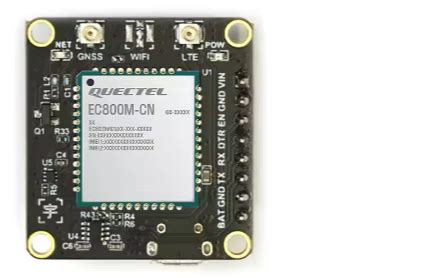
\includegraphics[width=0.5\textwidth]{QUECTEL_EC800M_CN.png}
		\caption{Module 4G LTE tích hợp GPS Quectel EC800K}
		\label{fig:ec800k}
	\end{figure}
	
	Hình 2.3 trên mô tả Module Quectel EC800KCNLC-I03-SNNSA là giải pháp kết nối 4G LTE và định vị GPS cho các ứng dụng IoT
	
	\subsubsection{Thông số kỹ thuật}
	\begin{table}[h]
		\centering
		\caption{Thông số kỹ thuật module EC800K}
		\label{tab:ec800k_specs}
		\begin{tabular}{|l|l|}
			\hline
			\textbf{Đặc tính} & \textbf{Thông số} \\ \hline
			Hỗ trợ mạng & LTE Cat 1 (10Mbps down/5Mbps up), 3G, 2G \\ \hline
			Băng tần LTE & FDD: B1/B3/B5/B8; TDD: B34/B38/B39/B40/B41 \\ \hline
			Định vị & GPS/GLONASS/Beidou, độ chính xác 2.5m \\ \hline
			Giao tiếp & UART, USB, GPIO \\ \hline
			Điện áp & 5V \\ \hline
			SMS & Hỗ trợ gửi/nhận \\ \hline
			Dữ liệu & 4G LTE (không VoLTE) \\ \hline
			Kích thước & 17.7×15.8×2.4mm \\ \hline
			Nhiệt độ & -35°C đến +75°C \\ \hline
		\end{tabular}
	\end{table}
	
	\subsubsection{Giao tiếp AT Command}
	\begin{itemize}
		\item Giao tiếp qua UART/USB với vi điều khiển (ESP32)
		\item Các lệnh AT cơ bản:
		\begin{itemize}
			\item \texttt{AT+CGPS=1} - Khởi động GPS
			\item \texttt{AT+CGPSINFO} - Lấy tọa độ GPS
			\item \texttt{AT+CMGS="+84..."} - Gửi SMS
			\item \texttt{AT+CNETLIGHT=1} - Điều khiển đèn báo
		\end{itemize}
	\end{itemize}
	
	\subsubsection{Kết nối với ESP32}
	\begin{table}[h]
		\centering
		\caption{Kết nối EC800K với ESP32}
		\label{tab:ec800k_connection}
		\begin{tabular}{|c|c|c|c|c|}
			\hline
			\textbf{Chân EC800K} & VCC & GND & TX & RX \\ \hline
			\textbf{Chân ESP32} & 5V & GND & RX (GPIO16) & TX (GPIO17) \\ \hline
		\end{tabular}
	\end{table}
	%PHẦN MỀM ------------------------------------------------------------------
	
	\section{Khung phát triển phần mềm}
	Nội dung phần này trình bày về các thành phần để sử dụng xây dựng nên mã nguồn của hệ thống phát hiện té ngã, phương pháp xử dữ liệu phát sinh từ cảm biến trong quá trình hoạt động để thực hiện yêu cầu đồ án
	\subsection{ESP-IDF Framework}
	ESP-IDF (Espressif IoT Development Framework) là môi trường phát triển chính thức cho ESP32, cung cấp đầy đủ công cụ để xây dựng ứng dụng nhúng. Framework này bao gồm:
	
	\subsubsection{Thành phần và các công cụ phát triển}
	\begin{itemize}
		\item \textbf{Công cụ phát triển}:
		\begin{itemize}
			\item Trình biên dịch GCC cho ESP32
			\item Hệ thống build CMake
			\item OpenOCD cho debug trực tiếp
		\end{itemize}
		
		\item \textbf{Thư viện phần mềm}:
		\begin{itemize}
			\item FreeRTOS cho quản lý đa nhiệm
			\item API Wi-Fi/Bluetooth
			\item Driver phần cứng (UART, SPI, I2C, GPIO)
		\end{itemize}
	\end{itemize}
	
	\subsubsection{Cấu trúc của một project điển hình gồm các thành phần sau}
	\begin{table}[h]
		\centering
		\caption{Cấu trúc thư mục ESP-IDF}
		\begin{tabular}{|l|l|}
			\hline
			\textbf{Thành phần} & \textbf{Mô tả} \\ \hline
			CMakeLists.txt & Cấu hình build hệ thống \\ \hline
			main/ & Ứng dụng chính (main.c) \\ \hline
			components/ & Thư viện tùy chỉnh \\ \hline
			build/ & File nhị phân đã biên dịch \\ \hline
		\end{tabular}
	\end{table}
	
	\newpage
	
	\subsection{Quy trình phát triển}
	\begin{enumerate}
		\item Cài đặt toolchain ESP-IDF
		\item Biên dịch bằng \texttt{idf.py build}
		\item Nạp firmware qua \texttt{idf.py flash}
		\item Debug với \texttt{idf.py monitor}
	\end{enumerate}
	
	\subsection{Thiết kế hệ thống phát hiện té ngã}
	Việc phát hiện té ngã dựa trên phân tích dữ liệu từ cảm biến gia tốc (MPU6050) nhằm nhận diện các chuyển động bất thường xảy ra đột ngột và có khả năng gây nguy hiểm, luồng xử lý dữ liệu sẽ diên ra như sau.
	
	
	\begin{itemize}
		\item \textbf{Thu thập dữ liệu}:
		\begin{itemize}
			\item Đọc giá trị gia tốc (ax,ay,az) và vận tốc góc (gx,gy,gz) từ MPU6050 qua I2C
			\item Tần số lấy mẫu 100Hz
		\end{itemize}
		
		\item \textbf{Tiền xử lý}:
		\begin{itemize}
			\item Lọc nhiễu bằng bộ lọc low-pass
			\item Tính toán đặc trưng:
			\begin{equation}
				A = \sqrt{a_x^2 + a_y^2 + a_z^2}
			\end{equation}
		\end{itemize}
		
		
		\item\textbf{Thuật toán phát hiện té ngã}
		Hệ thống sử dụng phương pháp đa tiêu chí:
		
		\begin{table}[h]
			\centering
			\caption{Tiêu chí phát hiện té ngã}
			\begin{tabular}{|l|l|l|}
				\hline
				\textbf{Tiêu chí} & \textbf{Ngưỡng} & \textbf{Mục đích} \\ \hline
				Gia tốc tổng & >2.5g & Phát hiện va chạm \\ \hline
				Thời gian bất động & >3s & Xác nhận té ngã \\ \hline
				Góc nghiêng & >45° & Loại bỏ cảnh báo giả \\ \hline
			\end{tabular}
		\end{table}
		
		
	\end{itemize}
	
	%CHAPTER3......................................... THIETKETHUCHIENPHANCUNG
	\chapter{THIẾT KẾ VÀ THỰC HIỆN PHẦN CỨNG}
	Chương nầy trình bày chi tiết việc chọn lựa và thực hiện thực tế sản phẩm dựa trên các phân tích và tìm hiểu lý thuyết của chương 2 vừa trình bày phía trên. Hệ thống phần cứng được xây dựng dựa trên ba thành phần cốt lõi: vi điều khiển ESP32 đảm nhiệm xử lý trung tâm, cảm biến MPU6050 để thu thập dữ liệu chuyển động, và module 4G EC800K cho kết nối không dây và định vị. Các giao tiếp chính bao gồm I2C cho cảm biến và UART cho module 4G.
	
	\section{Yêu cầu thiết kế của hệ thống phát hiện té ngã }
	
	
	Bảng \ref{tab:specs} dưới đây sẽ tổng kết các mô tả các yêu cầu kỹ thuật chính của hệ thống được đề ra
	
	\begin{table}[htbp]
		\centering
		\caption{Thông số kỹ thuật hệ thống}
		\label{tab:specs}
		\begin{tabular}{ll}
			\hline
			\textbf{Thông số} & \textbf{Yêu cầu} \\
			\hline
			Nguồn điện & 3.3V-5V DC hoặc pin Li-ion 3.7V \\
			Tiêu thụ năng lượng & Tối đa 500mA ở chế độ hoạt động \\
			Kích thước & ≤ 100×60×20mm \\
			Độ tin cậy & có khả năng hoạt Hoạt động liên tục trên 4h nếu bằng pin  \\
			
			\hline
		\end{tabular}
	\end{table}
	
	\section{Phân tích các phương án có thể thực hiện}
	
	\subsection{Tiêu chí đánh giá và so sánh các phương án}
	Các phương án thiết kế được đánh giá dựa trên bốn tiêu chí chính: (1) thời gian triển khai, (2) độ ổn định kết nối, (3) khả năng bảo trì, và (4) chi phí thực hiện. Mỗi tiêu chí được định lượng theo thang điểm từ 1-5 để so sánh khách quan.
	
	
	Bảng \ref{tab:design_options} dưới đây sẽ trình bày và phân tích chi tiết ba phương án thiết kế:
	
	\begin{table}[htbp]
		\centering
		\caption{So sánh các phương án thiết kế}
		\label{tab:design_options}
		\begin{tabular}{lccc}
			\hline
			\textbf{Tiêu chí} & \textbf{PCB} & \textbf{Breadboard} & \textbf{Board đục lỗ} \\
			\hline
			Thời gian triển khai & 2/5 & 5/5 & 4/5 \\
			Độ ổn định & 5/5 & 2/5 & 4/5 \\
			Chi phí ban đầu & 1/5 & 5/5 & 3/5 \\
			Khả năng mở rộng & 3/5 & 4/5 & 4/5 \\
			Phù hợp mục tiêu & 2/5 & 3/5 & 5/5 \\
			\hline
		\end{tabular}
	\end{table}
	
	\subsection{Phương án được lựa chọn theo tình hình thực tế}
	
	\begin{itemize}
		\item \textbf{ Phương án board đục lỗ }
		Phương án board đục lỗ được lựa chọn nhờ cân bằng giữa độ ổn định và tính linh hoạt. Thiết kế này cho phép hàn cố định các linh kiện chính (ESP32, MPU6050, EC800K) trên board FR-4 kích thước 80×50mm, sử dụng dây dẫn đồng 0.5mm² cho các kết nối giữa các module.
		\item \textbf{Giải pháp nguồn điện}   
		Hệ thống sử dụng nguồn có thể gồm pin Li-ion 18650 3.7V/2000mAh và nguồn DC 5V, cấp nguồn cho vi điều khiển và các modul cảm biến cũng nhu modul SIM
	\end{itemize}
	
	% ----------------
	
	\section{Sơ đồ khối tổng quát và thành phần của mạch phần cứng}
	
	\subsection{Tổng quan hệ thống}
	\begin{figure}[H]
		\centering
		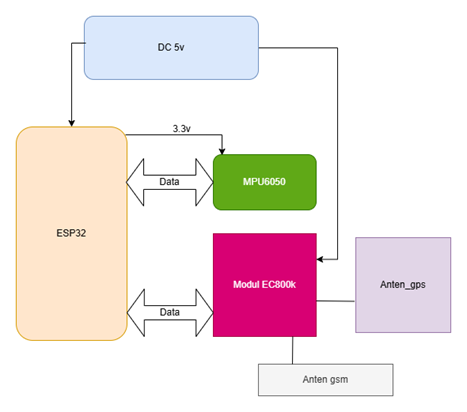
\includegraphics[width=0.95\textwidth]{SYSTEM_DIAGRAM.png}
		\caption{Sơ đồ khối tổng thể hệ thống}
		\label{fig:system_block}
	\end{figure}
	
	Hệ thống gồm 4 thành phần chính được thể hiện trong Hình \ref{fig:system_block}:
	\begin{enumerate}
		\item Khối nguồn với mạch chuyển đổi 5V sang 3.3V
		\item Vi điều khiển ESP32 xử lý trung tâm
		\item Cảm biến MPU6050 thu thập dữ liệu chuyển động
		\item Module EC800K tích hợp 4G/GPS
	\end{enumerate}
	
	\subsection{Các thành phần chi tiết}
	
	
	\subsubsection{Kết nối ESP32-MPU6050}
	\begin{figure}[H]
		\centering
		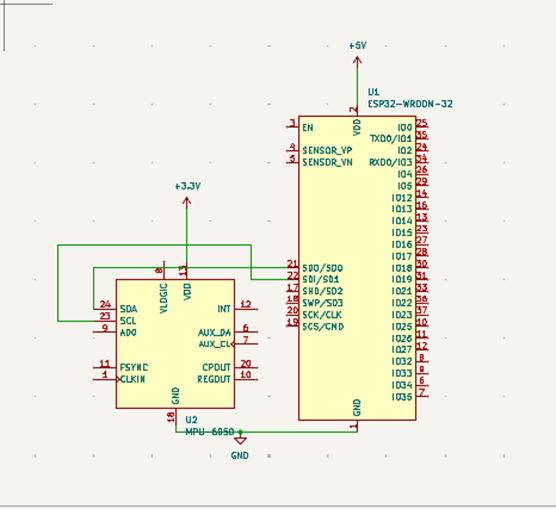
\includegraphics[width=0.7\textwidth]{ESP32_MPU6050_SCHEMATIC.png}
		\caption{Sơ đồ chân kết nối I2C}
		\label{fig:i2c_connection}
	\end{figure}
	
	Giao tiếp I2C giữa ESP32 và MPU6050 (Hình \ref{fig:i2c_connection}) sử dụng:
	\begin{itemize}
		\item Chân SDA (GPIO21)
		\item Chân SCL (GPIO22)
		\item Tần số hoạt động 400kHz
	\end{itemize}
	
	\subsubsection{Kết nối ESP32-EC800K}
	\begin{figure}[H]
		\centering
		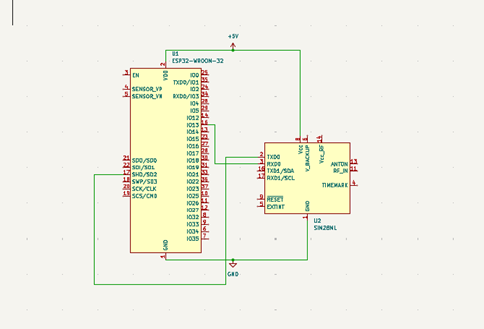
\includegraphics[width=0.8\textwidth]{ESP32_QUECTEL_EC800.png}
		\caption{Sơ đồ giao tiếp UART}
		\label{fig:uart_connection}
	\end{figure}
	
	Module EC800K giao tiếp với ESP32 qua UART (Hình \ref{fig:uart_connection}) với cấu hình:
	\begin{itemize}
		\item Baudrate 115200
		\item Chân TX (GPIO17)
		\item Chân RX (GPIO16)
		\item Flow control RTS/CTS
	\end{itemize}
	
	\subsection{Sơ đồ mạch hoàn chỉnh}
	\begin{figure}[H]
		\centering
		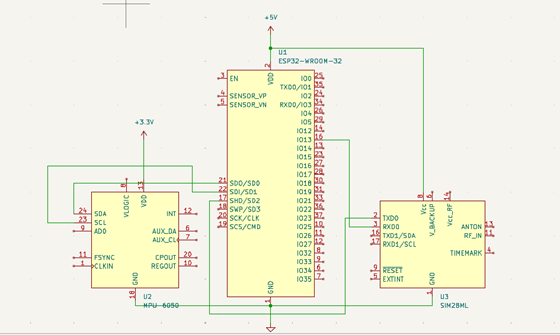
\includegraphics[width=\textwidth]{FULL_SCHEMATIC.png}
		\caption{Thiết kế mạch tổng thể}
		\label{fig:full_design}
	\end{figure}
	
	Toàn bộ các thành phần chân kết nối đượcnối với nhau như mạch schematic  (Hình \ref{fig:full_design}) :
	%   chuong 4----------------------------------
	
	
	\chapter{THIẾT KẾ VÀ THỰC HIỆN PHẦN MỀM}
	
	\section{Yêu cầu đặt ra cho phần mềm}
	
	\subsection{Các chức năng chính của phần mềm}
	
	Phần mềm hệ thống cần thực hiện ba chức năng cốt lõi: phát hiện té ngã thông qua phân tích dữ liệu từ cảm biến MPU6050, gửi cảnh báo khẩn cấp qua tin nhắn SMS kèm tọa độ GPS, và ghi nhật ký hoạt động để phục vụ cho việc giám sát và nâng cấp hệ thống. Cụ thể, hệ thống phải liên tục thu thập và xử lý dữ liệu gia tốc và vận tốc góc từ cảm biến, áp dụng thuật toán phát hiện té ngã dựa trên ngưỡng xác định trước, đồng thời duy trì khả năng phản ứng nhanh trong các tình huống khẩn cấp.
	
	Khi xác định có sự kiện té ngã, hệ thống sẽ kích hoạt hai cơ chế cảnh báo đồng thời: phát tín hiệu âm thanh qua buzzer để cảnh báo tại chỗ và gửi tin nhắn SMS chứa thông tin vị trí chính xác đến số điện thoại được cấu hình sẵn. Quá trình này đòi hỏi sự phối hợp nhịp nhàng giữa các module phần cứng thông qua các giao thức truyền thông khác nhau, bao gồm I2C cho cảm biến, UART cho module SIM 4G, và GPIO để điều khiển các thiết bị ngoại vi.
	
	\subsection{Yêu cầu về hiệu suất và tiết kiệm năng lượng}
	
	Về hiệu suất, hệ thống cần đảm bảo khả năng xử lý dữ liệu cảm biến trong thời gian thực với độ trễ tối thiểu. Thuật toán phát hiện té ngã phải được tối ưu để vừa đảm bảo độ chính xác cao, vừa phù hợp với khả năng tính toán của vi điều khiển ESP32. Đặc biệt quan trọng là cơ chế quản lý năng lượng thông minh, bao gồm việc áp dụng các chế độ ngủ sâu (deep sleep) khi hệ thống không hoạt động và tối ưu hóa chu kỳ lấy mẫu cảm biến để kéo dài thời gian sử dụng pin.
	
	\subsection{Yêu cầu về giao diện người dùng}
	
	Hệ thống được thiết kế với giao diện người dùng tối giản, tập trung vào tính năng tự động hóa cao. Các thông số cấu hình như số điện thoại nhận cảnh báo sẽ được thiết lập trực tiếp trong mã nguồn, cho phép người dùng có kiến thức kỹ thuật cơ bản có thể dễ dàng tùy chỉnh thông qua việc chỉnh sửa các hằng số trong file cấu hình. Quá trình vận hành hệ thống hoàn toàn tự động, không yêu cầu tương tác thường xuyên từ người dùng.
	
	\section{Phân tích và thiết kế kiến trúc phần mềm}
	
	\subsection{Phương pháp phát hiện té ngã}
	
	Thuật toán phát hiện té ngã được xây dựng dựa trên phương pháp ngưỡng động lực học kết hợp, sử dụng cả dữ liệu gia tốc và vận tốc góc. Hệ thống sẽ xác định sự kiện té ngã khi đồng thời thỏa mãn hai điều kiện: độ lớn gia tốc tổng hợp vượt quá ngưỡng 2.5g và vận tốc góc vượt quá 200°/s. Phương pháp này giúp giảm thiểu cảnh báo sai trong các trường hợp vận động mạnh thông thường.
	
	\subsection{Tổ chức mã nguồn}
	
	Hệ thống được phát triển theo kiến trúc module hóa trên nền tảng ESP-IDF, với cấu trúc thư mục được thiết kế khoa học để dễ dàng bảo trì và mở rộng, cho phép tách biệt rõ ràng các chức năng, với mỗi module đảm nhiệm một nhiệm vụ cụ thể. File main.c đóng vai trò điều phối chính, trong khi các module con xử lý các tác vụ chuyên biệt như giao tiếp cảm biến, xử lý GPS, và quản lý log hệ thống. Cách tổ chức này không chỉ nâng cao khả năng bảo trì mà còn tạo điều kiện thuận lợi cho việc phát triển các tính năng mới trong tương lai.
	
	Hệ thống sử dụng FreeRTOS để quản lý các tác vụ đồng thời một cách hiệu quả. Các tác vụ chính bao gồm: đọc cảm biến (ưu tiên cao), xử lý phát hiện té ngã, quản lý truyền thông, và ghi log (ưu tiên thấp). Cơ chế semaphore và queue được áp dụng để đảm bảo đồng bộ dữ liệu giữa các tác vụ, đồng thời tối ưu hóa việc sử dụng tài nguyên hệ thống.
	
	\newpage
	\begin{verbatim}
		mainproject/
		│
		├── main/
		│   └── main.c                     // Khởi tạo hệ thống, tạo các task chính
		│
		├── components/
		│   ├── mpu6050/                   // Giao tiếp và xử lý dữ liệu MPU6050
		│   │   ├── mpu6050.c
		│   │   └── mpu6050.h
		│   │
		│   ├── sim4g_gps/                 // Module xử lý lấy GPS và gửi SMS
		│   │   ├── sim4g_gps.c
		│   │   └── sim4g_gps.h
		│   │
		│   ├── comm/                      // Quản lý UART, I2C, GPIO
		│   │   ├── comm.c
		│   │   └── comm.h
		│   │
		│   └── debugs/                    // Ghi log, kiểm tra hệ thống
		│       ├── debugs.c
		│       └── debugs.h
		│
		└── CMakeLists.txt                 // Cấu hình build cho toàn bộ dự án
	\end{verbatim}
	
	%chương tiep theo ------------------------------------
	
	
	\section{Lưu đồ giải thuật tổng quát và giải thích}
	
	\begin{figure}[h]
		\centering
		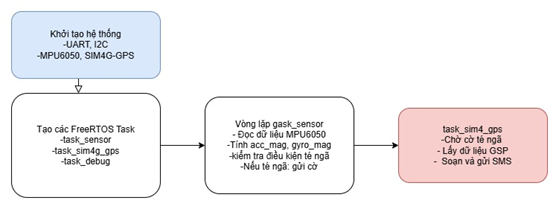
\includegraphics[width=\textwidth]{luu_do_phan_mem.png}
		\caption{Lưu đồ phần mềm}
		\label{fig:software_flowchart}
	\end{figure}
	
	\begin{figure}[h]
		\centering
		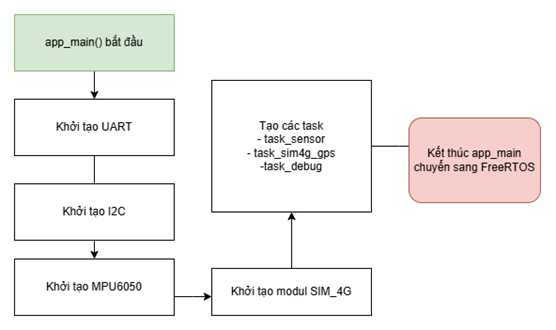
\includegraphics[width=\textwidth]{luu_do_phan_app_main.png}
		\caption{Lưu đồ phần app\_main()}
		\label{fig:app_main_flowchart}
	\end{figure}
	
	Dự án được xây dựng theo kiến trúc phần mềm phân lớp, sử dụng hệ thống component của ESP-IDF để chia tách các chức năng thành từng module riêng biệt. Việc tổ chức phần mềm theo cấu trúc này giúp tăng tính tái sử dụng, dễ dàng bảo trì, kiểm thử và mở rộng trong tương lai. Cấu trúc chính bao gồm thư mục \texttt{main/} chứa chương trình chính, và thư mục \texttt{components/} bao gồm các module chức năng riêng biệt.
	
	\subsection{Thư mục main}
	
	Chứa chương trình chính với hàm \texttt{app\_main()}. Đây là điểm khởi đầu của chương trình, có nhiệm vụ khởi tạo toàn bộ hệ thống như giao tiếp UART, I2C, cảm biến MPU6050, module SIM 4G-GPS. Ngoài ra, trong \texttt{app\_main()} còn tạo và quản lý các tác vụ riêng biệt (FreeRTOS task) cho các chức năng như xử lý cảm biến, truyền thông với module 4G, hoặc ghi log. Hàm main không thực hiện các xử lý chi tiết mà gọi đến các hàm đã được tách riêng ở các module tương ứng trong \texttt{components/}.
	
	\subsection{Module mpu6050}
	
	Thực hiện việc giao tiếp I2C với cảm biến MPU6050. Đọc dữ liệu gia tốc và con quay hồi chuyển từ cảm biến, tính toán độ lớn tổng hợp của các vector gia tốc và gyro. Dựa vào ngưỡng định sẵn, module này đưa ra quyết định về việc có xảy ra té ngã hay không.
	
	\textbf{Thành phần:}
	\begin{itemize}
		\item \texttt{mpu6050.c}: Cài đặt các hàm khởi tạo cảm biến, đọc và xử lý dữ liệu.
		\item \texttt{mpu6050.h}: Khai báo các hàm API công khai để module khác sử dụng.
		\item \texttt{CMakeLists.txt}: Định nghĩa thông tin biên dịch riêng cho module.
	\end{itemize}
	
	\subsection{Module sim4g\_gps}
	
	Giao tiếp với module Quectel EC800K thông qua UART, gửi các tập lệnh AT để: Lấy thông tin định vị GPS (qua các lệnh như \texttt{AT+CGNSINF}). Gửi tin nhắn SMS đến số điện thoại đã cấu hình sẵn trong mã nguồn khi phát hiện té ngã. Quản lý trạng thái module SIM, kiểm tra mạng và tín hiệu.
	
	\textbf{Thành phần:}
	\begin{itemize}
		\item \texttt{sim4g\_gps.c}: Cài đặt các hàm giao tiếp và xử lý tập lệnh AT.
		\item \texttt{sim4g\_gps.h}: Khai báo API công khai.
		\item \texttt{CMakeLists.txt}: Tập tin biên dịch riêng.
	\end{itemize}
	
	\subsection{Module comm}
	
	Cung cấp các hàm khởi tạo và giao tiếp phần cứng thấp như UART, I2C và GPIO. Module này đóng vai trò trung gian để các module khác (ví dụ \texttt{mpu6050}, \texttt{sim4g\_gps}) sử dụng mà không cần trực tiếp thao tác với các hàm cấp thấp của ESP-IDF.
	
	\textbf{Thành phần:}
	\begin{itemize}
		\item \texttt{comm.c}: Cài đặt hàm khởi tạo UART, I2C và thao tác GPIO.
		\item \texttt{comm.h}: Khai báo API công khai.
		\item \texttt{CMakeLists.txt}: Tập tin biên dịch riêng.
	\end{itemize}
	
	\subsection{Module debugs}
	
	Ghi log trạng thái hệ thống ra UART0. Giúp người phát triển có thể theo dõi trạng thái hoạt động của cảm biến, module 4G và hệ thống nói chung trong quá trình thử nghiệm và vận hành.
	
	\textbf{Thành phần:}
	\begin{itemize}
		\item \texttt{debugs.c}: Cài đặt hàm ghi log và in trạng thái hệ thống.
		\item \texttt{debugs.h}: Khai báo API công khai.
		\item \texttt{CMakeLists.txt}: Tập tin biên dịch riêng.
	\end{itemize}
	
	\newpage
	
	\section{Lưu đồ giải thuật chi tiết và giải thích}
	
	Khi phát hiện được sự kiện té ngã, hệ thống sẽ kích hoạt module sim4g\_gps để thực hiện việc gửi cảnh báo. Module này giao tiếp với EC800K qua AT command để lấy tọa độ GPS chính xác và gửi tin nhắn SMS cảnh báo kèm theo thông tin vị trí đến số điện thoại đã được cấu hình sẵn trong hệ thống. Như 2 lưu đồ được miêu tả trong hình 4.3 và 4.4 dưới đây
	\begin{figure}[h]
		\centering
		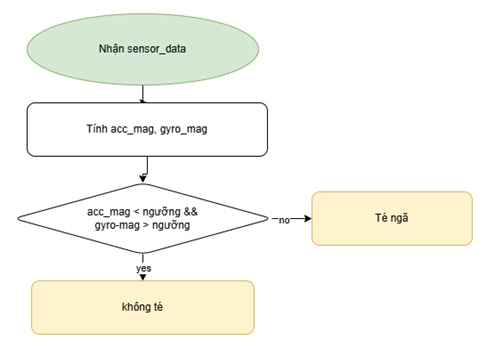
\includegraphics[width=\textwidth]{luu_do_phat_hien_te_nga_don_gian.png}
		\caption{Lưu đồ thuật toán phát hiện té ngã đơn giản}
		\label{fig:fall_detection_algorithm}
	\end{figure}
	
	\begin{figure}[h]
		\centering
		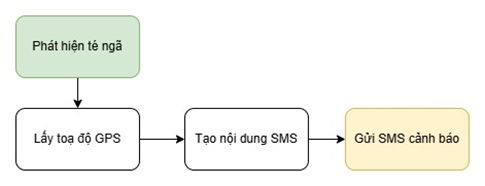
\includegraphics[width=\textwidth]{luu_do_gui_canh_bao_dinh_vi_gps.png}
		\caption{Lưu đồ gửi cảnh báo và định vị GPS}
		\label{fig:gps_alert_flowchart}
	\end{figure}
	
	
	
	%--------------- ket qua thuc hien
	
	\chapter{KẾT QUẢ THỰC HIỆN}
	Chương này là chương trình bày kế quả đạt được sau khi kết hợp phần mềm và phần cứng thành sản phẩm thực tế
	\section{Các thành phần linh kiện và cách thức hoàn thành sản phẩm thực tế}
	
	\subsection{Thành phần phần cứng thực tế}
	
	Hệ thống được cung cấp nguồn điện thông qua adapter 5V cấp qua cổng USB hoặc pin Li-ion 3.7V thông qua mạch sạc, đảm bảo tính linh hoạt trong việc sử dụng. Các chân GPIO của ESP32 được cấu hình cẩn thận trong mã nguồn để xử lý các tín hiệu từ các module, tạo nên một hệ thống hoàn chỉnh và ổn định. hình từ 5.1 tới 5.4 là hình ảnh thực của các thành phần linh kiện
	
	\begin{figure}[h]
		\centering
		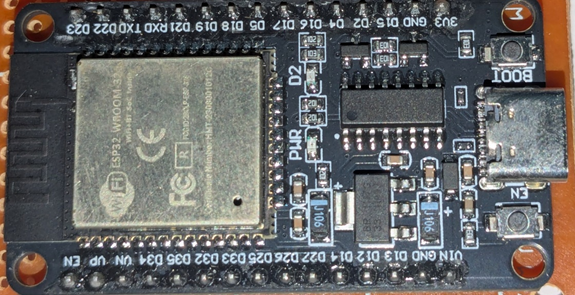
\includegraphics[width=0.7\textwidth]{real_mainboar-esp32.png}
		\caption{Bo mạch chính: ESP32 DevKit V1}
		\label{fig:esp32_devkit}
	\end{figure}
	
	\vspace{2cm}
	
	\begin{figure}[h]
		\centering
		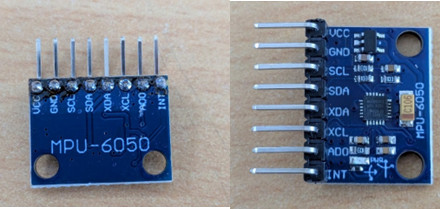
\includegraphics[width=0.7\textwidth]{real_6050.png}
		\caption{Cảm biến: MPU6050 (giao tiếp I2C)}
		\label{fig:mpu6050_sensor}
	\end{figure}
	
	\vspace{2cm} 
	
	\begin{figure}[h]
		\centering
		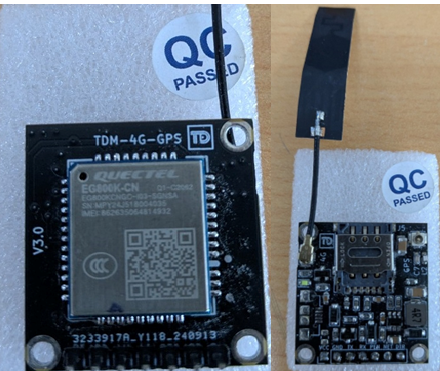
\includegraphics[width=0.7\textwidth]{real_sim_modul.png}
		\caption{Module: Quectel EC800K (giao tiếp UART)}
		\label{fig:quectel_module}
	\end{figure}
	
	\newpage
	\subsection{Kết quả phần cứng thực tế }
	
	\begin{figure}[h]
		\centering
		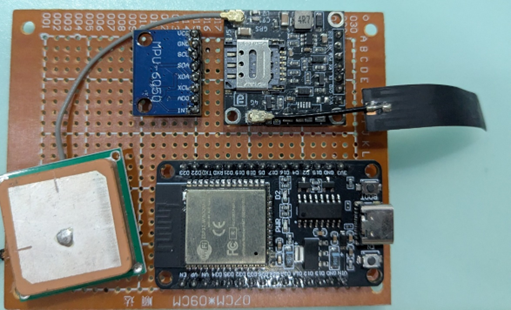
\includegraphics[width=0.8\textwidth]{real_composed_mainboard_upside.png}
		\caption{Hình ảnh sản phẩm hoàn thiện}
		\label{fig:final_product}
	\end{figure}
	
	
	\subsection{Công cụ phần mềm được sử dụng}
	
	\begin{itemize}
		\item \textbf{Draw.IO}: Vẽ sơ đồ khối
		\item \textbf{Kicad}: Vẽ mạch schematic
		\item \textbf{ESP-IDF v5.x}: Nền tảng phát triển chính cho ESP32
		\item \textbf{Vim và Sublime Text}: Các công cụ để viết mã nguồn
		\item \textbf{Terminal + idf.py}: Dùng để biên dịch, nạp chương trình và giám sát log
		\item \textbf{Python}: Sử dụng trong môi trường ESP-IDF IDE để hỗ trợ các công cụ biên dịch và giám sát
	\end{itemize}
	
	\textbf{Các bước tiến hành thử nghiệm:}
	\begin{enumerate}
		\item \textbf{Lập trình ESP32}: Nạp chương trình vào ESP32 qua lệnh \texttt{idf.py flash monitor}.
		\item \textbf{Giả lập tình huống té ngã}: Lắc mạnh hoặc thả rơi nhẹ thiết bị để kích hoạt cảm biến MPU6050 và phát hiện té ngã.
		\item \textbf{Quan sát log hệ thống}: Sử dụng \texttt{idf.py monitor} để theo dõi log và xác nhận sự kiện té ngã được phát hiện.
		\item \textbf{Kiểm tra tính năng gửi cảnh báo}: Đảm bảo rằng hệ thống gửi tin nhắn SMS với tọa độ GPS chính xác tới số điện thoại đã cấu hình.
		\item \textbf{Lặp lại thử nghiệm}: Thực hiện nhiều lần để kiểm tra độ chính xác và ổn định của hệ thống, bao gồm độ nhạy cảm của cảm biến và khả năng gửi tin nhắn đúng thời gian.
	\end{enumerate}
	
	\newpage
	
	\section{Trình bày số liệu thu được từ log của phần mềm khi thử nghiệm}
	
	Số liệu đo đạc từ cảm biến MPU6050 được thu thập trong hai tình huống khác nhau: khi có sự kiện té ngã và khi thiết bị hoạt động bình thường. Dữ liệu này cho phép so sánh và phân tích để xác định ngưỡng phát hiện chính xác.
	
	\begin{table}[h]
		\centering
		\caption{Dữ liệu trong tình huống té ngã}
		\label{tab:fall_data}
		\begin{tabular}{|c|c|c|c|c|c|c|c|}
			\hline
			\textbf{Gyro X} & \textbf{Gyro Y} & \textbf{Gyro Z} & \textbf{Gyro Mag} & \textbf{Accel X} & \textbf{Accel Y} & \textbf{Accel Z} & \textbf{Accel Mag} \\
			\textbf{(deg/s)} & \textbf{(deg/s)} & \textbf{(deg/s)} & \textbf{(deg/s)} & \textbf{(g)} & \textbf{(g)} & \textbf{(g)} & \textbf{(g)} \\
			\hline
			129.60 & -36.77 & 29.19 & 137.84 & 0.65 & 0.79 & -0.79 & 1.29 \\
			-43.90 & 214.79 & 52.97 & 225.54 & 0.53 & 2.00 & -2.00 & 2.88 \\
			158.75 & 250.13 & 134.18 & 325.22 & -1.18 & 1.72 & 1.56 & 2.61 \\
			-250.14 & -246.07 & -250.14 & 430.91 & 1.11 & 2.00 & -2.00 & 3.04 \\
			242.56 & 250.13 & 250.13 & 428.91 & -1.33 & -2.00 & 2.00 & 3.13 \\
			-11.60 & -146.43 & -169.58 & 224.35 & 1.80 & 2.00 & -2.00 & 3.35 \\
			201.32 & 238.97 & 250.13 & 400.25 & -2.00 & 0.21 & 2.00 & 2.84 \\
			-250.14 & -250.14 & -250.14 & 433.25 & 0.55 & 0.23 & -0.37 & 0.69 \\
			\hline
		\end{tabular}
	\end{table}
	
	\begin{table}[h]
		\centering
		\caption{Dữ liệu trong tình huống bình thường}
		\label{tab:normal_data}
		\begin{tabular}{|c|c|c|c|c|c|c|c|}
			\hline
			\textbf{Gyro X} & \textbf{Gyro Y} & \textbf{Gyro Z} & \textbf{Gyro Mag} & \textbf{Accel X} & \textbf{Accel Y} & \textbf{Accel Z} & \textbf{Accel Mag} \\
			\textbf{(deg/s)} & \textbf{(deg/s)} & \textbf{(deg/s)} & \textbf{(deg/s)} & \textbf{(g)} & \textbf{(g)} & \textbf{(g)} & \textbf{(g)} \\
			\hline
			1.27 & -1.46 & 0.51 & 2.00 & -0.03 & 0.01 & -0.96 & 0.96 \\
			1.07 & -0.95 & 0.53 & 1.52 & -0.04 & 0.02 & -0.97 & 0.97 \\
			1.18 & -1.36 & 0.73 & 1.94 & -0.03 & 0.02 & -0.97 & 0.97 \\
			1.03 & -1.02 & 0.40 & 1.50 & -0.03 & 0.01 & -0.97 & 0.97 \\
			1.37 & -1.08 & 0.58 & 1.84 & -0.03 & 0.01 & -0.97 & 0.97 \\
			0.77 & -0.83 & 0.47 & 1.23 & -0.03 & 0.01 & -0.97 & 0.97 \\
			1.02 & -0.37 & 0.77 & 1.33 & -0.03 & 0.01 & -0.97 & 0.97 \\
			\hline
		\end{tabular}
	\end{table}
	
	\begin{table}[h]
		\centering
		\caption{Bảng kết quả thu được từ log test của modul 4g\_gps}
		\label{tab:gps_data}
		\begin{tabular}{|c|c|c|c|c|c|c|}
			\hline
			\textbf{Time (UTC)} & \textbf{Latitude} & \textbf{Longitude} & \textbf{Altitude (m)} & \textbf{Fix Mode} & \textbf{Date} & \textbf{Satellites} \\
			\hline
			132517.00 & 1053.3115N & 10646.7839E & 5.07 & 3 & 240425 & 07 \\
			132517.00 & 1053.3115N & 10646.7839E & 5.07 & 3 & 240425 & 07 \\
			132540.00 & 1053.3117N & 10646.7840E & 5.05 & 3 & 240425 & 07 \\
			132540.00 & 1053.3117N & 10646.7840E & 5.05 & 3 & 240425 & 07 \\
			132627.00 & 1053.3107N & 10646.7839E & 5.02 & 3 & 240425 & 07 \\
			132627.00 & 1053.3107N & 10646.7839E & 5.02 & 3 & 240425 & 07 \\
			\hline
		\end{tabular}
	\end{table}
	
	\newpage 
	
	\section{Giải thích và phân tích về kết quả thu được}
	
	\begin{table}[h]
		\centering
		\caption{So sánh dữ liệu té ngã và không té ngã}
		\label{tab:comparison}
		\begin{tabular}{|l|c|c|}
			\hline
			\textbf{Thông số} & \textbf{Trung bình té ngã} & \textbf{Trung bình bình thường} \\
			\hline
			Gyro X (deg/s) & 22.06 & 1.10 \\
			Gyro Y (deg/s) & 34.33 & -1.03 \\
			Gyro Z (deg/s) & 5.84 & 0.57 \\
			Gyro Mag (deg/s) & 325.78 & 1.63 \\
			Accel X (g) & 0.02 & -0.03 \\
			Accel Y (g) & 0.87 & 0.01 \\
			Accel Z (g) & -0.20 & -0.97 \\
			Accel Mag (g) & 2.48 & 0.97 \\
			\hline
		\end{tabular}
	\end{table}
	
	Từ bảng so sánh trên có thể thấy sự khác biệt rõ rệt giữa hai trạng thái. Các giá trị gia tốc và tốc độ quay trong tình huống té ngã thường cao đột biến so với trạng thái bình thường, đặc biệt là độ lớn gia tốc (Accel Mag) và độ lớn góc quay (Gyro Mag) có thể dùng làm tiêu chí phát hiện té ngã hiệu quả.
	
	\textbf{Phân tích số liệu từ modul 4G-GPS:} Tín hiệu GPS thu được liên tục với chế độ định vị hoạt động (QGPS: 1), số lượng vệ tinh dao động từ 07 vệ tinh trở lên cho phép định vị chính xác. Vị trí GPS thay đổi theo thời gian nhưng rất gần nhau, chứng tỏ thiết bị đang di chuyển tuyến tính và chậm. Dữ liệu mạng (CSQ = 31,99) cho thấy cường độ tín hiệu mạng di động mạnh, tuy nhiên trạng thái đăng ký mạng (CREG: 0,0) cho thấy chưa đăng ký mạng thành công do chưa lắp sim.
	
	Thời gian phản hồi của hệ thống hoạt động đúng theo như cài đặt ban đầu. Phân tích độ chính xác của hệ thống cho thấy kết quả phù hợp với yêu cầu đề ra từ ban đầu, đảm bảo tính tin cậy và ứng dụng thực tế.
	
	\chapter{KẾT LUẬN VÀ HƯỚNG PHÁT TRIỂN}
	
	\section{Kết luận}
	Hệ thống đã đạt được những kết quả quan trọng trong việc phát hiện té ngã thông qua phân tích dữ liệu từ cảm biến gia tốc và vận tốc góc. Ưu điểm nổi bật là thiết kế đơn giản, chi phí thấp và khả năng hoạt động thời gian thực. Tuy nhiên, hệ thống vẫn tồn tại một số hạn chế như tỷ lệ phát hiện sai trong môi trường nhiễu cao và tiêu thụ năng lượng chưa tối ưu. So với mục tiêu ban đầu, hệ thống đáp ứng được yêu cầu cơ bản nhưng cần cải tiến để nâng cao độ chính xác và hiệu quả năng lượng.
	
	\section{Hướng phát triển}
	
	\subsection{Cải tiến phần cứng}
	Về phần cứng, hệ thống có thể được nâng cấp trên nhiều khía cạnh. Đầu tiên, việc cải thiện hiệu suất năng lượng có thể thực hiện bằng cách sử dụng module cảm biến với chế độ tự động ngủ (sleep mode) và thay thế pin Li-ion bằng nguồn năng lượng hiệu quả hơn như pin mặt trời. 
	Độ chính xác của hệ thống có thể được nâng cao thông qua việc thay thế cảm biến MPU6050 bằng các phiên bản cao cấp hơn như MPU9250 hoặc LSM9DS1. Module GPS cũng cần được nâng cấp để hỗ trợ thêm các hệ thống định vị như Galileo hay GLONASS, giúp tăng độ chính xác của dữ liệu vị trí.
	
	Thiết kế phần cứng cần hướng đến sự nhỏ gọn hơn bằng cách tích hợp tất cả thành phần (cảm biến, GPS, ESP32) vào một bo mạch duy nhất. Có thể bổ sung thêm các module phụ trợ như màn hình LCD, còi báo động hoặc camera để tăng tính tiện ích.
	
	\subsection{Cải tiến phần mềm}
	Về phần mềm, thuật toán phát hiện té ngã hiện tại dựa trên ngưỡng gia tốc đơn giản có thể được thay thế bằng các giải thuật machine learning phức tạp hơn để giảm thiểu tỷ lệ báo động sai. Hệ thống cần tích hợp thêm khả năng kết nối 4G/5G không chỉ để gửi cảnh báo mà còn hỗ trợ điều khiển từ xa và báo cáo trạng thái. Việc tối ưu hóa năng lượng ở mức phần mềm cũng rất quan trọng, bao gồm việc đưa vi điều khiển vào chế độ Deep Sleep khi không hoạt động.
	
	Giao diện người dùng cần được phát triển thông qua ứng dụng di động hoặc web, cho phép cấu hình thông số hệ thống và theo dõi trạng thái thiết bị trực quan hơn. Ứng dụng này có thể tích hợp bản đồ số để hiển thị vị trí người dùng khi xảy ra sự cố.
	
	\chapter{TÀI LIỆU THAM KHẢO}
	
	\begin{enumerate}
		\item M. Casilari, R. Luque, and A. Morón, "Fall detection systems based on machine learning models trained with wearable inertial sensors: A review," \textit{Expert Systems with Applications}, vol. 223, 2023. [Online]. Available: \url{https://www.sciencedirect.com/science/article/abs/pii/S095219762300177X}
		
		\item J. Zhang, X. Liu, and S. Wang, "Design of an interactive fall detection system for smart home care using depth cameras," \textit{Journal of Computer-Aided Design \& Computer Graphics}, vol. 35, no. 3, pp. 350–358, 2023. [Online]. Available: \url{https://www.jcad.cn/en/article/doi/10.3724/SP.J.1089.2023.20050}
		
		\item Apple Inc., “Use fall detection with Apple Watch,” \textit{Apple Support}, [Online]. Available: \url{https://support.apple.com/en-us/108896}
		
		\item Philips Lifeline, “GoSafe 2 User Manual,” \textit{Manualslib}, [Online]. Available: \url{https://www.manualslib.com/manual/1536831/Philips-Lifeline-Gosafe-2.html}
		
		\item MobileHelp, “MobileHelp Solo,” \textit{MobileHelp Official Site}, [Online]. Available: \url{https://www.mobilehelp.com/products/mobilehelp-solo/}
		
		\item Milesight, “VS373 AI Workplace Occupancy Sensor,” \textit{Milesight IoT}, [Online]. Available: \url{https://www.milesight.com/iot/product/lorawan-sensor/vs373}
		
		\item Vayyar Imaging, “Radar applications: The potential of 4D imaging,” \textit{Vayyar Blog}, [Online]. Available: \url{https://vayyar.com/blog/vayyar/radar-applications-the-potential-of-4d-imaging/}
		
		\item ASUS, “Zenbo Junior – Smart Robot for Education and Care,” \textit{ASUS Support}, [Online]. Available: \url{https://www.asus.com/support/faq/1039870/}
		
		\item Nobi, “Smart Lamp for Fall Detection and Elderly Care,” \textit{Nobi Official Site}, [Online]. Available: \url{https://www.nobi.life/en}
		
		\item FallCall Solutions, “FallCall Detect,” \textit{App Store}, [Online]. Available: \url{https://apps.apple.com/us/app/fallcall-detect/id1547299584}
		
		\item Essence Group, “SmartCare Platform,” \textit{Essence SmartCare}, [Online]. Available: \url{https://www.essencesmartcare.com/solutions/smartcare-solutions/}
	\end{enumerate}
	
	\section*{Mã nguồn chương trình chính}
	Mã nguồn chương trình chính được upload lên trang Github cá nhân của sinh viên thực hiện đề tài \\
	
	\url{https://github.com/wikibird2024/mainproject/tree/master}
	
	
\end{document}